\documentclass{article}

\usepackage{amsmath,amssymb}
\usepackage{tikz}
\usepackage{pgfplots}
\usepackage{xcolor}
\usepackage[left=2.1cm,right=3.1cm,bottom=3cm,footskip=0.75cm,headsep=0.5cm]{geometry}
\usepackage{enumerate}
\usepackage{enumitem}
\usepackage{marvosym}
\usepackage{tabularx}
\usepackage{tikz-qtree}
\usetikzlibrary{patterns,arrows,calc,decorations.pathmorphing,backgrounds, positioning,fit,petri,decorations.fractals,trees,cd,automata,babel,shapes.geometric,arrows.meta,bending}

\usepackage[utf8]{inputenc}

\renewcommand*{\arraystretch}{1.4}

\newcolumntype{L}[1]{>{\raggedright\arraybackslash}p{#1}}
\newcolumntype{R}[1]{>{\raggedleft\arraybackslash}p{#1}}
\newcolumntype{C}[1]{>{\centering\let\newline\\\arraybackslash\hspace{0pt}}m{#1}}

\title{\textbf{Steuertheorie, Hausaufgabe 3}}
\author{\textsc{Henry Haustein}}
\date{}

\begin{document}
	\maketitle
	
	\section*{Aufgabe 1}
	\begin{enumerate}[label=(\alph*)]
		\item falsch, denn es gibt keinen Wohlfahrtsverlust
		\begin{center}
			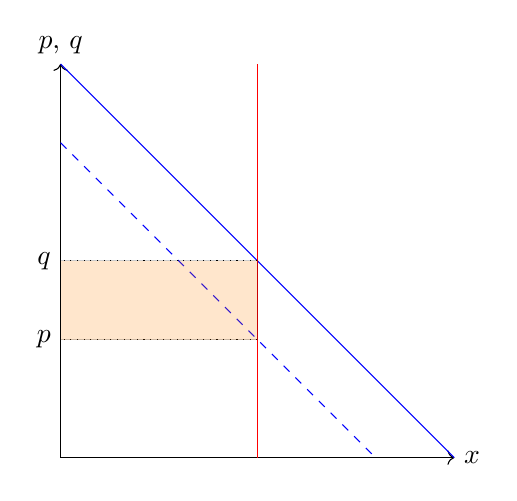
\begin{tikzpicture}
				\draw[->] (0,0) -- (5,0) node[right] {$x$};
				\draw[->] (0,0) -- (0,5) node[above] {$p$, $q$};
				
				\draw[blue] (0,5) -- (5,0);
				\draw[blue,dashed] (0,4) -- (4,0);
				\draw[red] (2.5,0) -- (2.5,5);
				
				\draw[dotted] (2.5,2.5) -- (0,2.5) node[left] {$q$};
				\draw[dotted] (2.5,1.5) -- (0,1.5) node[left] {$p$};
				
				\draw[fill=orange,opacity=0.2] (0,2.5) rectangle (2.5,1.5);
			\end{tikzpicture} \\
			\textcolor{blue}{GZB ohne/mit Steuern}, \textcolor{red}{Angebot}, \textcolor{orange}{Steueraufkommen}
		\end{center}
		\item falsch, es gibt Nullgewinne vor und nach der Maßnahme:
		\begin{align}
			\Pi_{vor} &= p_0x_0 - GKx_0 \notag \\
			&= GKx_0 - GKx_0 = 0 \notag \\
			\Pi_{nach} &= p_1x_1 - (GK-s)x_1 \notag \\
			&= (GK-s)x_1 - (GK-s)x_1 = 0 \notag
		\end{align}
		\begin{center}
			\begin{tikzpicture}
				\draw[->] (0,0) -- (5,0) node[right] {$x$};
				\draw[->] (0,0) -- (0,5) node[above] {$p$, $q$};
				
				\draw[blue] (0,5) -- (5,0);
				\draw[blue,dashed] (0,4) -- (4,0);
				\draw[red] (0,2) -- (5,2);
				\draw[red, dashed] (0,1) -- (5,1);
				
				\draw[dotted] (3,0) node[below] {$x_0$, $x_1$} -- (3,2);
				\draw[dotted] (0,2) -- (0,2) node[left] {$p_0$};
				\draw[dotted] (0,1) -- (0,1) node[left] {$p_1$};
			\end{tikzpicture} \\
			\textcolor{blue}{GZB ohne/mit Steuern}, \textcolor{red}{GK ohne/mit Subvention}
		\end{center}
		\item richtig, Einbuße = Steueraufkommen + Wohlfahrtsverlust
		\begin{center}
			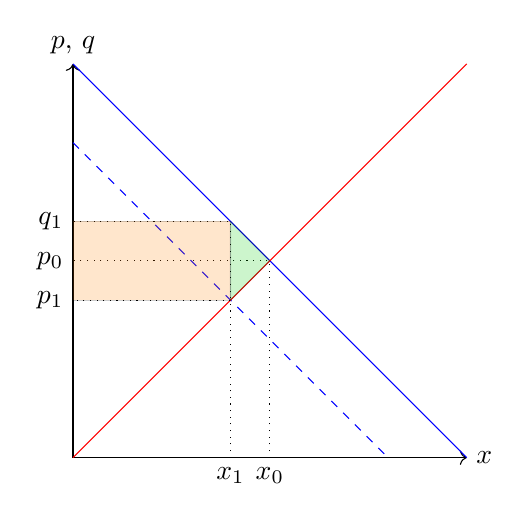
\begin{tikzpicture}
				\draw[->] (0,0) -- (5,0) node[right] {$x$};
				\draw[->] (0,0) -- (0,5) node[above] {$p$, $q$};
				
				\draw[blue] (0,5) -- (5,0);
				\draw[blue,dashed] (0,4) -- (4,0);
				\draw[red] (0,0) -- (5,5);
				
				\draw[dotted] (2.5,0) node[below] {$x_0$} -- (2.5,2.5) -- (0,2.5) node[left] {$p_0$};
				\draw[dotted] (2,0) node[below] {$x_1$} -- (2,3) -- (0,3) node[left] {$q_1$};
				\draw[dotted] (2,2) -- (0,2) node[left] {$p_1$};
				
				\draw[fill=orange, opacity=0.2] (0,3) rectangle (2,2);
				\draw[fill=green!80!black,opacity=0.2] (2,3) -- (2,2) -- (2.5,2.5) -- (2,3);
			\end{tikzpicture} \\
			\textcolor{blue}{Nachfrage ohne/mit Steuern}, \textcolor{red}{Angebot}, \textcolor{green!80!black}{Wohlfahrtsverlust}, \textcolor{orange}{Steueraufkommen}
		\end{center}
	\end{enumerate}

	\section*{Aufgabe 2}
	\begin{enumerate}[label=(\alph*)]
		\item Diagramm
		\begin{center}
			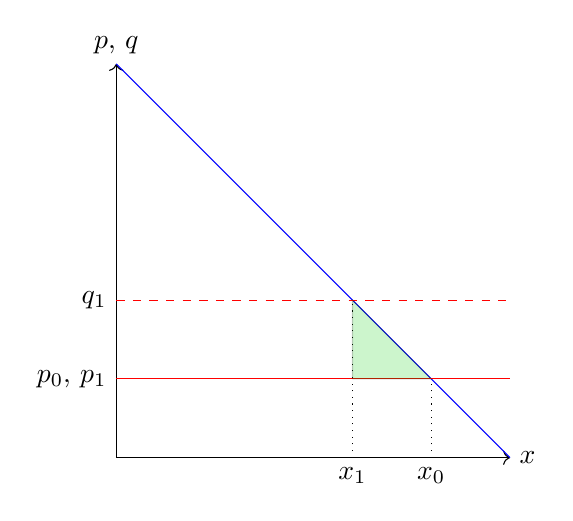
\begin{tikzpicture}
				\draw[->] (0,0) -- (5,0) node[right] {$x$};
				\draw[->] (0,0) -- (0,5) node[above] {$p$, $q$};
				
				\draw[blue] (0,5) -- (5,0);
				\draw[red,dashed] (0,2) -- (5,2);
				\draw[red] (0,1) -- (5,1);
				
				\draw[dotted] (4,0) node[below] {$x_0$} -- (4,1);
				\draw[dotted] (3,0) node[below] {$x_1$} -- (3,2);
				\draw[dotted] (0,2) -- (0,2) node[left] {$q_1$};
				\draw[dotted] (0,1) -- (0,1) node[left] {$p_0$, $p_1$};
				
				\draw[fill=green!80!black,opacity=0.2] (3,1) -- (4,1) -- (3,2) -- (3,1);
			\end{tikzpicture} \\
			\textcolor{blue}{GZB}, \textcolor{red}{GK ohne/mit Steuern}, \textcolor{green!80!black}{Wohlfahrtsverlust}
		\end{center}
		\item ohne Steuern
		\begin{align}
			GZB &= Gk \notag \\
			20-x &= 5 \notag \\
			x_0 &= 15 \Rightarrow p_0 = 5 \notag
		\end{align}
		mit Steuern
		\begin{align}
			GZB &= GK + t \notag \\
			20-x &= 5+4 \notag \\
			x_1 &= 11 \Rightarrow q_1=9\Rightarrow p_1=5 \notag
		\end{align}
		\item Der Wohlfahrtsverlust beträgt
		\begin{align}
			WFV &= \frac{1}{2}(x_0-x_1)(q_1-p_0) \notag \\
			&= \frac{1}{2}(15-11)(9-5) \notag \\
			&= 8 \notag
		\end{align}
		\item Das Steueraufkommen ist $T=x_1\cdot t=11\cdot 4=44$.
		\item Diagramm
		\begin{center}
			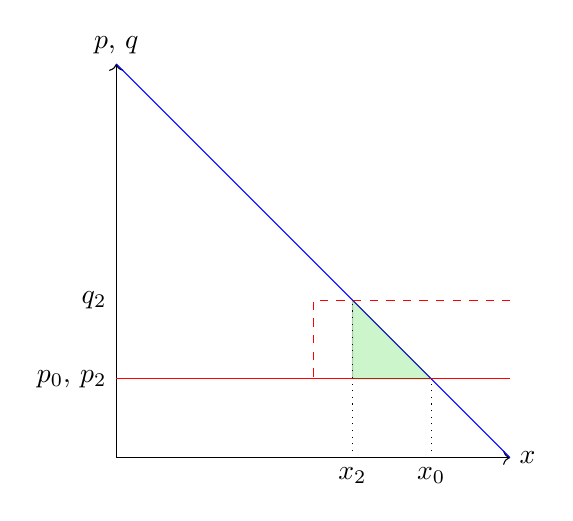
\begin{tikzpicture}
				\draw[->] (0,0) -- (5,0) node[right] {$x$};
				\draw[->] (0,0) -- (0,5) node[above] {$p$, $q$};
				
				\draw[blue] (0,5) -- (5,0);
				\draw[red,dashed] (0,1) -- (2.5,1) -- (2.5,2) -- (5,2);
				\draw[red] (0,1) -- (5,1);
				
				\draw[dotted] (4,0) node[below] {$x_0$} -- (4,1);
				\draw[dotted] (3,0) node[below] {$x_2$} -- (3,2);
				\draw[dotted] (0,2) -- (0,2) node[left] {$q_2$};
				\draw[dotted] (0,1) -- (0,1) node[left] {$p_0$, $p_2$};
				
				\draw[fill=green!80!black,opacity=0.2] (3,1) -- (4,1) -- (3,2) -- (3,1);
			\end{tikzpicture} \\
			\textcolor{blue}{GZB}, \textcolor{red}{GK ohne/mit Steuern}, \textcolor{green!80!black}{Wohlfahrtsverlust}
		\end{center}
		\item Da Mengen und Preise gleich bleiben, ändert sich auf der Wohlfahrtsverlust nicht.
		\item $T=(x_2-9)\cdot t=2\cdot 4=8$.
	\end{enumerate}

	\section*{Aufgabe 3}
	\begin{enumerate}[label=(\alph*)]
		\item Es handelt sich hier um Cobb-Douglas-Präferenzen, das heißt es werden 50 \% des Einkommens für Gut 1 und Gut 2 ausgegeben:
		\begin{align}
			x_1 &= \frac{\frac{1}{2}E}{p_x} = \frac{8}{2} = 4 \notag \\
			y_1 &= \frac{\frac{1}{2}E}{p_y} = \frac{8}{2} = 4 \notag
		\end{align}
		\item Es gibt einen neuen Preis für Gut 1: $q_x=(1+\theta)p_x = 4$. Damit gilt
		\begin{align}
			x_2 &= \frac{\frac{1}{2}E}{q_x} = \frac{8}{4} = 2 \notag \\
			y_2 &= \frac{\frac{1}{2}E}{p_y} = \frac{8}{2} = 4 \notag
		\end{align}
		Das Steueraufkommen ist $T=x_2\cdot \theta\cdot p_x = 2\cdot 1\cdot 2=4$.
		\item Die Steuer und das Steueraufkommen kann man hier nicht in Geldeinheiten ablesen, sondern nur in Einheiten von $y$.
		\begin{center}
			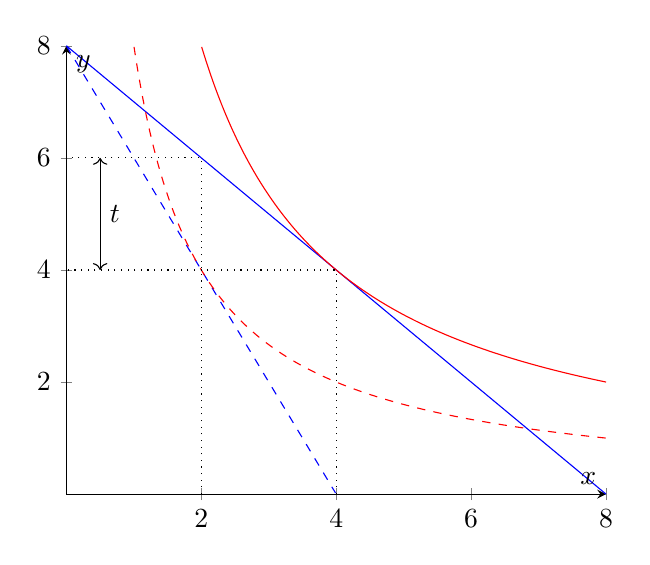
\begin{tikzpicture}
				\begin{axis}[
					xmin=0, xmax=8, xlabel=$x$,
					ymin=0, ymax=8, ylabel=$y$,
					samples=400,
					axis x line=middle,
					axis y line=middle,
					domain=0:8,
					restrict y to domain=0:8
					]
					\addplot[mark=none,smooth,blue] {8-x};
					\addplot[mark=none,smooth,blue,dashed] {8-2*x};
					\addplot[mark=none,smooth,red] {16/x};
					\addplot[mark=none,smooth,red,dashed] {8/x};
					
					\draw[dotted] (axis cs: 4,0) -- (axis cs: 4,4) -- (axis cs: 0,4);
					\draw[dotted] (axis cs: 2,0) -- (axis cs: 2,6) -- (axis cs: 0,6);
					\draw[<->] (axis cs: 0.5,4) to node[midway,right] {$t$} (axis cs: 0.5,6);
					
				\end{axis}
			\end{tikzpicture} \\
			\textcolor{blue}{Budgetrestriktion vor/nach Besteuerung}, \textcolor{red}{Nutzenniveaus vor/nach Besteuerung}
		\end{center}
		\item Eine Pauschalsteuer wirkt wie eine Einkommensreduktion. Das neue Einkommen ist $E_2=E-t=16-4=12$. Damit ist die Nachfrage
		\begin{align}
			x_3 &= \frac{\frac{1}{2}E_2}{p_x} = \frac{6}{2} = 3 \notag \\
			y_3 &= \frac{\frac{1}{2}E_2}{p_y} = \frac{6}{2} = 3 \notag
		\end{align}
		\item Ein Vergleich der Nutzen nach Besteuerung zeigt, dass das selbe Steueraufkommen zu einem höheren Nutzen bei Pauschalsteuer erzeugt werden kann:
		\begin{align}
			U_{\theta_x} &= \sqrt{2}\cdot \sqrt{4} = 2\sqrt{2} \approx 2.828 \notag \\
			U_{Pauschal} &= \sqrt{3}\cdot\sqrt{3} = 3 \notag
		\end{align}
		\begin{center}
			\begin{tikzpicture}
				\begin{axis}[
					xmin=0, xmax=8, xlabel=$x$,
					ymin=0, ymax=8, ylabel=$y$,
					samples=400,
					axis x line=middle,
					axis y line=middle,
					domain=0:8,
					restrict y to domain=0:8
					]
					\addplot[mark=none,smooth,blue] {8-x};
					\addplot[mark=none,smooth,blue,dashed] {6-x};
					\addplot[mark=none,smooth,red] {16/x};
					\addplot[mark=none,smooth,red,dashed] {9/x};
					
					\draw[dotted] (axis cs: 4,0) -- (axis cs: 4,4) -- (axis cs: 0,4);
					\draw[dotted] (axis cs: 3,0) -- (axis cs: 3,3) -- (axis cs: 0,3);
					
				\end{axis}
			\end{tikzpicture} \\
			\textcolor{blue}{Budgetrestriktion vor/nach Besteuerung}, \textcolor{red}{Nutzenniveaus vor/nach Besteuerung}
		\end{center}
	\end{enumerate}

	\section*{Aufgabe 4}
	\begin{center}
		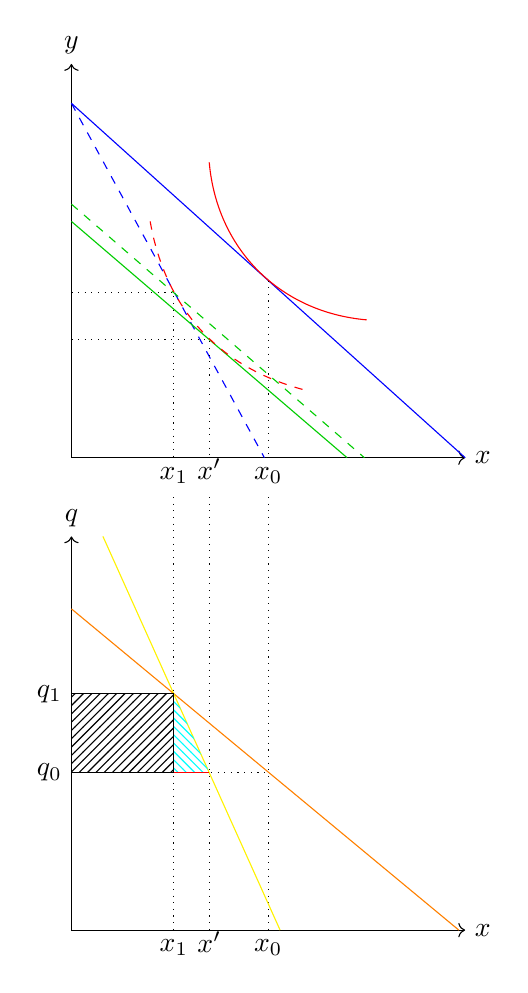
\begin{tikzpicture}
			\draw[->] (0,0) -- (5,0) node[right] {$x$};
			\draw[->] (0,0) -- (0,5) node[above] {$y$};
			
			\draw[blue] (0,4.5) -- (5,0);
			\draw[blue,dashed] (0,4.5) -- (2.45,0);
			\draw[green!80!black] (0,3) -- (3.5,0);
			\draw[green!80!black,dashed] (0,3.22) -- (3.72,0);
			
			\draw[red] (1.75,3.75) to[bend right=40] (3.75,1.75);
			\draw[red,dashed] (1,3) to[bend right=33] (3,0.85);
			
			\draw[dotted] (0,2.1) -- (1.3,2.1) to (1.3,0) node[below] {$x_1$};
			\draw[dotted] (0,1.5) -- (1.75,1.5) to (1.75,0) node[below,yshift=3] {$x'$};
			\draw[dotted] (2.5,2.25) to (2.5,0) node[below] {$x_0$};
			
			\draw[->] (0,-6) -- (5,-6) node[right] {$x$};
			\draw[->] (0,-6) -- (0,-1) node[above] {$q$};
			
			\draw[dotted] (1.3,-0.5) to (1.3,-6) node[below] {$x_1$};
			\draw[dotted] (1.75,-0.5) to (1.75,-6) node[below,yshift=3] {$x'$};
			\draw[dotted] (2.5,-0.5) to (2.5,-6) node[below] {$x_0$};
			
			\draw[orange] (0,-1.92) -- (4.92,-6);
			\draw[yellow] (0.4,-1) -- (2.65,-6);
			
			\draw[dotted] (0,-3) node[left] {$q_1$} -- (1.3,-3);
			\draw[dotted] (0,-4) node[left] {$q_0$} -- (2.5,-4);
			
			\draw[red,pattern=north west lines, pattern color=cyan] (1.3,-3) -- (1.3,-4) -- (1.75,-4) (1.3,-3);
			\draw[pattern=north east lines, pattern color=black] (0,-4) rectangle (1.3,-3);
		\end{tikzpicture} \\
		\textcolor{orange}{$D_M$}, \textcolor{yellow}{$D_H$}, fiktives Steueraufkommen, falls der Haushalt durch den Staat für die Steuererhebung kompensiert würde, \textcolor{cyan}{Excess Burden}
	\end{center}

	\section*{Aufgabe 5}
	\begin{enumerate}[label=(\alph*)]
		\item Wir haben wieder Cobb-Douglas-Präferenzen, das heißt es werden 50 \% des Einkommens für Gut 1 und für Gut 2 ausgegeben. Vor der Besteuerung gilt
		\begin{align}
			x_1^1 &= \frac{\frac{1}{2}m}{p_1^1} = \frac{50}{1} = 50 \notag \\
			x_2^1 &= \frac{\frac{1}{2}m}{p_2^1} = \frac{50}{2} = 25 \notag \\
			U^1 &= x_1^1 \cdot x_2^1 = 50\cdot 25 = 1250 \notag
		\end{align}
		Nach der Besteuerung gilt
		\begin{align}
			x_1^2 &= \frac{\frac{1}{2}m}{p_1^2} = \frac{50}{4} = 12.5 \notag \\
			x_2^2 &= \frac{\frac{1}{2}m}{p_2^2} = \frac{50}{2} = 25 \notag \\
			U^2 &= x_1^2 \cdot x_2^2 = 12.5\cdot 25 = 312.5 \notag
		\end{align}
		\item Es gilt
		\begin{align}
			U^2 &= x_1 \cdot x_2 \notag \\
			&= \frac{\frac{1}{2}m^{AV}}{p_1^1} \cdot \frac{\frac{1}{2}m^{AV}}{p_2^1} \notag \\
			&= \frac{1}{2}m^{AV} \cdot \frac{1}{4}m^{AV} \notag \\
			&= \frac{1}{8}\left(m^{AV}\right)^2 \notag \\
			m^{AV} &= \sqrt{8\cdot U^2} \notag \\
			&= \sqrt{8\cdot 312.5} \notag \\
			&= 50 \notag
		\end{align}
		Die äquivalente Variation ist also $AV=m-m^{AV}=50$. Der Haushalt ist also bereit 50 Geldeinheiten an den Staat zu zahlen, damit dieser auf die Besteuerung verzichtet.
		\item Für die Wertsteuer $\theta$ gilt: $p_1^2 = 4 = (1+\theta)\cdot p_1^1$ $\Rightarrow$ $\theta=3$. Damit ist das Steueraufkommen
		\begin{align}
			T = x_1^2 \cdot\theta \cdot p_1^1 = 12.5\cdot 3\cdot 1 = 37.5 \notag
		\end{align}
		Der Excess Burden ist $AV - T = 50-37.5=12.5$.
		\item Es gilt
		\begin{align}
			U^1 &= \frac{\frac{1}{2}m^{KV}}{p_1^2} \cdot\frac{\frac{1}{2}m^{KV}}{p_2^2} \notag \\
			&= \frac{1}{8}m^{KV}\cdot \frac{1}{4}m^{KV} \notag \\
			&= \frac{1}{32}\left(m^{KV}\right)^2 \notag \\
			m^{KV} &= \sqrt{32\cdot U^1} \notag \\
			&= \sqrt{32\cdot 1250} \notag \\
			&= 200 \notag
		\end{align}
		Die kompensierende Variation ist also $KV=m^{KV}-m=200-100=100$. Der Staat müsste 100 Geldeinheiten zahlen, damit der Haushalt nach Steuern das gleiche Nutzenniveau wie vor Steuern hat.
		\item Das Steueraufkommen ist
		\begin{align}
			T = \frac{\frac{1}{2}m^{KV}}{p_1^2} \cdot \theta = 25\cdot 3 \notag
		\end{align}
		Der Excess Burden ist $KV-T=100-75=25$.
	\end{enumerate}
	
\end{document}